We consider the initial graph $G$ with vertices $v$ such that this neighborhood does not form a clique i.e $cliq(v) = -1$. 
We suggest an algorithm which modify the initial set $E_C$ by adding or deleting edges in order to get a {\em linegraph}. 
%Given that labeled vertices $v$ to $cliq(v) = -1$ in a given order $z_1 , z_2 , ..., z_t$. 
Given that vertices $v$ are labeled to $cliq(v) = -1$ in a given order $z_1 , z_2 , ..., z_t$. 
Let $E_C^i$ be the edge set of $G$ after the (i-1)-th vertices had been already treated in that order.  
In the following chapter, we denote by  $z = z_i$  a vertex and by ${\cal C}^{i}$ the set of cliques of $G_C$ at the i-th step. Thus $E_C^1 = E_C$ et ${\cal C} = {\cal C}^{1}$.

Let  $C(z) = \{C_1 , . . . , C_k \}$ be a set of all cliques from ${\cal C}^{i}$ of size at least 3 which  $z$ belongs to. 
We notice that the intersection of each pair of cliques from $C(z)$ gives the vertex $z$. 
We define by $S(z)$ the union of a set of all adjacent vertices $v$ of $z$ in the cliques $K_2 = \{v, z\} \in {\cal C}^i$ of size $2$ and a set of all adjacent vertices $v$ of $z$ such that $[v, z]$ is not covered by any clique of ${\cal C}^i$. 

\begin{equation}	
S(z) = \{ v \in \Gamma_{G}(z) | \{z,v\} \in C^i \} \cup \{ v \in \Gamma_{G}(z) | \{z,v\} \notin E(c), \forall c \in {\cal C}^i\}
\end{equation} 
with $E(c)$, an edge set of clique $c$.

\begin{definition}
Two cliques $C$ and $C'$ from ${\cal C}(z)$ are  {\bf contractables} if any edge $[u,v]$  of $E_C^i$ such that $u \in C$ and $v \in C'$ is not covered  by a clique (other that $\{u,v\}$) in ${\cal C}$. 
\end{definition}


\begin{definition}
A clique $C \in {\cal C}^i$ is {\bf neighbour} of $z$ if $C \notin {\cal C}(z)$ and $card(C \cap S(z)) \ge 2$.
The dependency of a clique $C$ neighbour of $z$ is the set $D_{z}(C) \subset {\cal C}(z)$ such as $C' \in D_{z}(C) $ and $C' \cap C \cap \Gamma_{G}(z) \ne \emptyset$.
A clique $C$ is {\bf increasing} if and only if it is neighbour of $z$ and $D_{z}(C)$ is contractable or empty.
\begin{equation}
voisine(z) = \{C \in {\cal C}^i \mbox{ } | \mbox{ } C \notin C(z) \mbox{ } \& \mbox{ } card(C \cap S(z)) \ge 2 \} \newline
\end{equation}
\begin{equation}
D_{z}(C) = \{ C' \in C(z) \mbox{ }|  \mbox{ } C' \cap C \cap \Gamma_{G}(z) \ne \emptyset \}
\end{equation}

\end{definition}

We denote by an \textbf{increasement} of $z$, an union of 
a vertex $\{z\}$, 
an increasing clique $C$ of $z$ and 
a contraction of cliques of $D_{z}(C)$.

\begin{definition}
We denote by a {\bf compression} de $z$, a triplet $T$ represented by $\pi_1$, $\pi_2$, $\pi_s$  defined by: 
	
\begin{itemize}	
	\item  $\pi_1$ (resp. $\pi_2$) can be one of two forms:
	\begin{enumerate} 		
		\item $\pi_1$ (respectively $\pi_2$) is the union of $\{z\}$, a subset $C_1$ (resp. $C_2$) of cliques from  ${\cal C}(z)$ such as any pair $C$ and $C'$ of $C_1$ (resp. $C_2$) is contractable and a subset $S_1$ (resp. $S_2$) of vertices $v \in S(z)$ not belonging to any clique such as:			
$$ \forall v \in S_1,~\forall x \in C_1, \not\exists C' \in {\cal C}~t.q.~card(C')>2~~et~~\{v,x\} \subset C'$$			
		\item $\pi_1$ (resp. $\pi_2$)  is an increasement of $z$.
	\end{enumerate}
	\item  $\pi_1$ and $\pi_2$ can not be simultaneously reduce to $\{z\}$ and  $\pi_1 \cap \pi_2 = \{z\}$.
	\item $\pi_S=\Gamma_G(z)-~((\pi_1 \cap \Gamma_G(z)) \cup(\pi_2 \cap \Gamma_G(z)))$ such as edge set $\{[z,v]\in E_{C}^{i}:~v\in \pi_S\}$  is not disconnecting. 	
	\item the triplet $\pi_{1} \cap \Gamma_{G}(z)$, $\pi_{2} \cap \Gamma_{G}(z)$, $\pi_{S} \cap \Gamma_{G}(z)$ is a 3-partition of $\Gamma_{G}(z)$.
\end{itemize}

\end{definition}


Such a compression always consists for example in whether 
$\pi_1 = \{z\} \cup C_i \in C(z)$, 
$\pi_2 =  \emptyset$,
$\pi_s = \gamma_G(z) -(\gamma_G(z) \cup C_i) $  if ${\cal C}(z)$ is not empty.
Else, 
$\pi_1 = \{z\} \cup \{ v \in \gamma_G(z)  \} $, 
$\pi_2 =  \emptyset$,
$\pi_s = \gamma_G(z) - \{v\} $
is an another compression.
Another example compression is given in the figure \ref{correctionGraph}.
\begin{centering} 
\begin{figure}[htb!]
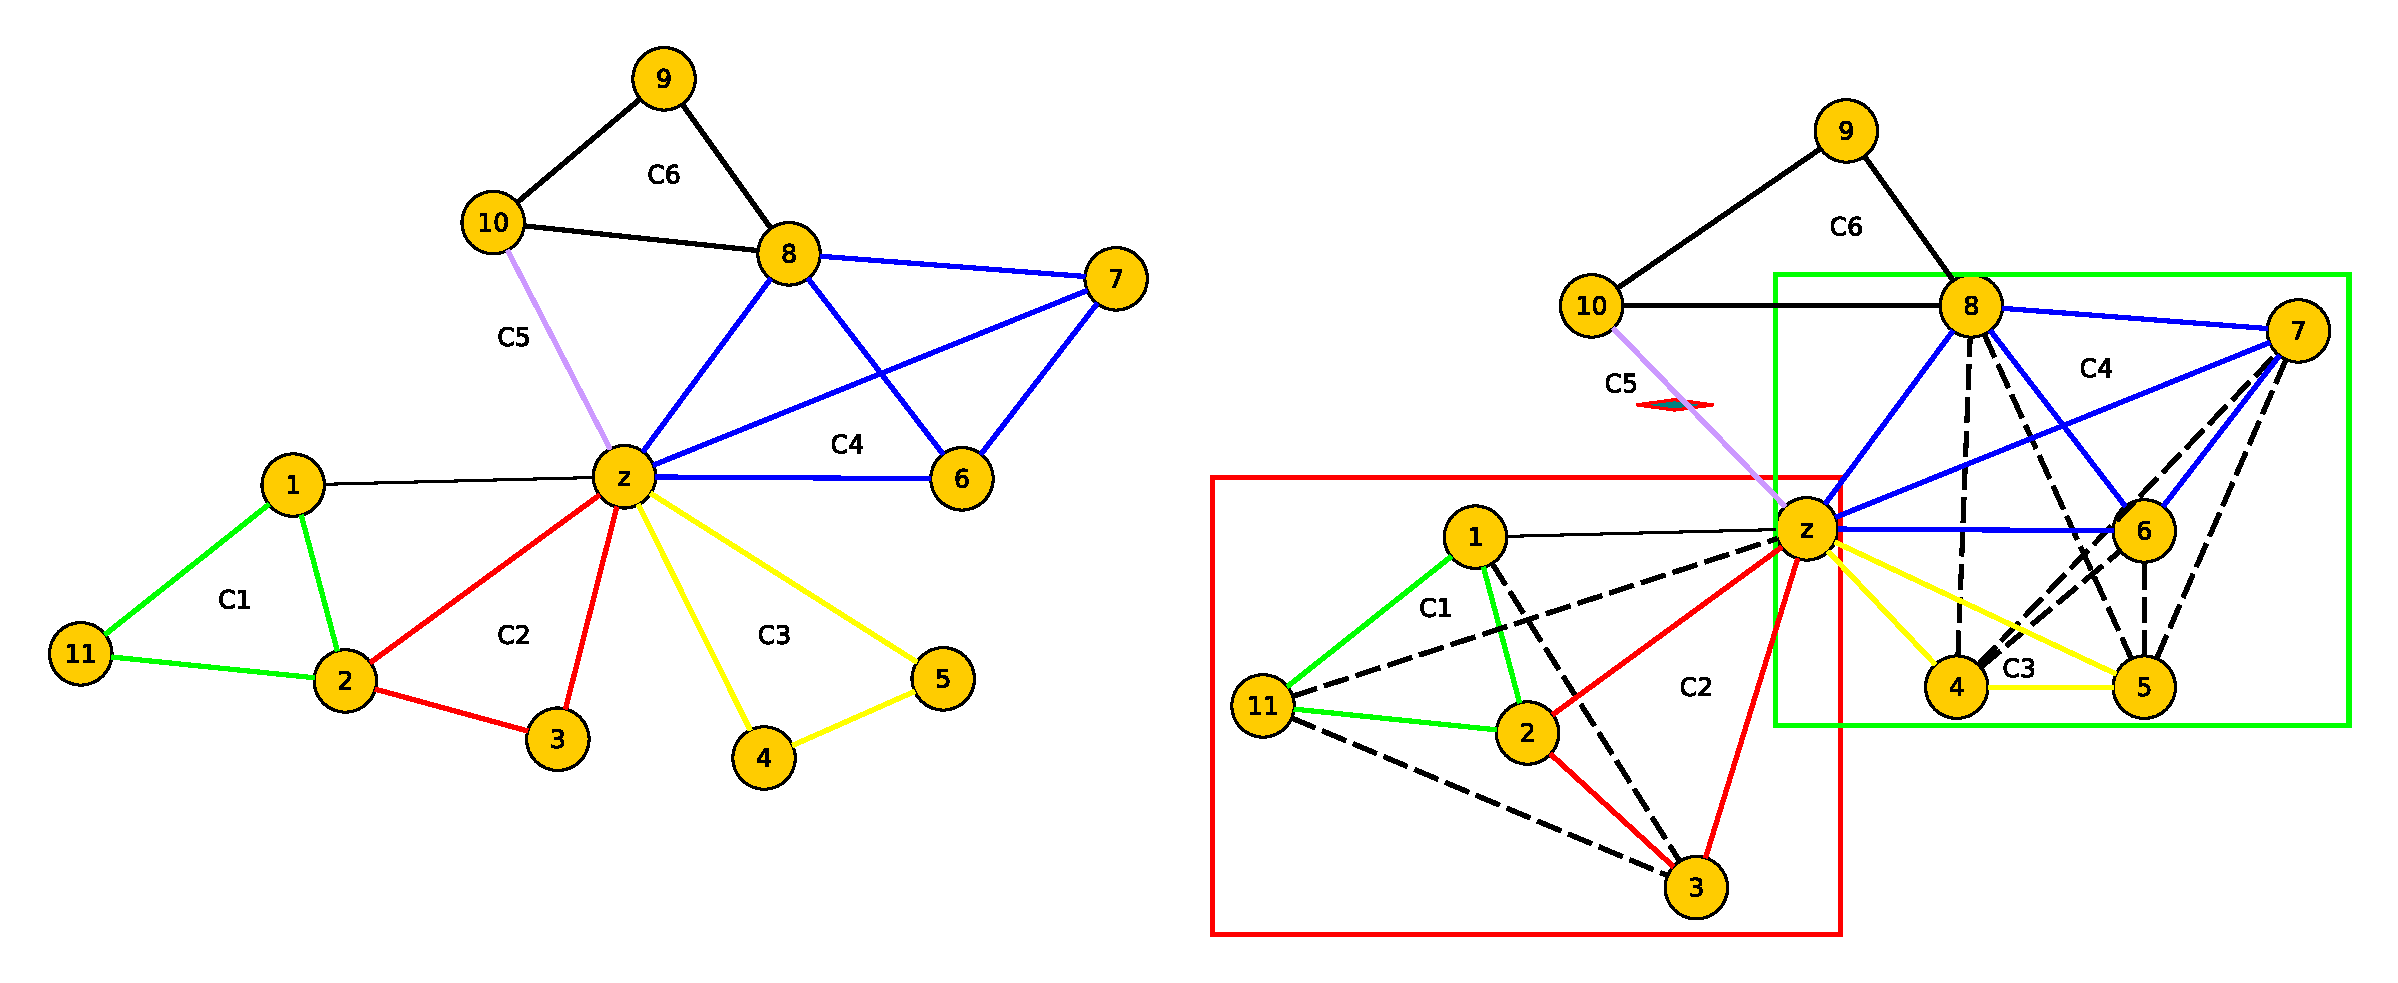
\includegraphics[scale=0.30]{./imagesLineGraphes/correctionGraph.eps} \vspace{-0.5em}
\caption{an compression example}
\label{correctionGraph}
\end{figure}
\end{centering} 


The $\pi_{1},\pi_{2},\pi_{S}$ compression cost is defined by:
$$c(T) = | \{\{u,v\} \in \pi_{1}:~[u,v]\not\in E_{C}^{i}\}| + |\{\{u,v\} \in \pi_2:~[u,v]\not\in E_{C}^{i}\}| +~ |\pi_S| $$



%Let $Cost(z)$ the minimum compression cost of $v$.
Let $Cost(z)$ be the minimum cost of a correlation cover of $v$. 

Our goal is to modify $G_C$ such as $z$ will be covered by one or two cliques from $\pi_1$ and $\pi_2$.
To do this, the cost of this change $ c(T) $ takes into account the edges to add (linked to $\pi_1$ and $\pi_2$) and to remove (linked to $\pi_S$).


Thus, {\bf applying a compression} $T=\pi_1,\pi_2,\pi_s$ consists in adding in $E_0$ the edges defined by the sets $\{\{u,v\} \in \pi_1:~[u,v]\not\in E_{C}^{i}\}$ (would be covered by the clique $\pi_1$) and $\{\{u,v\} \in \pi_2:~[u,v]\not\in  E_{C}^{i}\}$ (would be covered by the clique $\pi_2$), and to delete the edges $\{[z,v] \in  E_{C}^{i}:~v\in \pi_S\}$. 
From then on, vertex $z$ belongs to two cliques $\pi_1$ et $\pi_2$. 
We realize the following updates to obtain ${\cal C}^{i+1}$ and $E_{C}^{i+1}$ :

\begin{itemize} 
	\item delete all cliques ${\cal C}_z$ covered by $\pi_1$ in  ${\cal C}^{i}$.
	\item delete all cliques of cardinal $2$ covered by  $\pi_1$ and  $\pi_2$ in ${\cal C}^{i}$,        
	\item add $\pi_1$ and $\pi_2$ in ${\cal C}^{i}$, delete from $E^{i}_C$ all edges $\{[z,v] \in E_C^{i}:~v\in \pi_S\}$. 
	\item assign $Cliq(z)$ to $1$ (if $\pi_1$ or $\pi_2$ is empty) or $2$ (else).
\end{itemize}

This procedure has the following properties:
\begin{property}
We consider a compression operation.
Let ${\cal C}^{i+1}$ the set obtained from ${\cal C}^{i}$ after a compression.
\begin{enumerate}
\item each edge of $G_{C}$ covered by one or two cliques in ${\cal C}^{i}$ remains in ${\cal C}^{i+1}$.
\item each edge covered by only one clique in ${\cal C}^{i}$ and not deleted in ${\cal C}^{i}$  remains in ${\cal C}^{i+1}$.
\item the vertex $z$ is covered by one or two cliques in ${\cal C}^{i+1}$ (the number of vertices covered increases by $1$ compared to the number in ${\cal C}^{i}$).
\end{enumerate}
\end{property}

Thus, for each vertex $z_i$ of list $z_1, z_2, \ldots, z_t$ taken in that order, we consider a minimum compression cost $c_{m}^{i}$ and we apply it.
The property above ensure at the end of process, we obtain a correlation graph $G_{C}^{t} = (V, E_{C}^{t})$ whose the modified set $\cal C$ is a correlation cover.
The line-distance verifies $DL( G_{C}^{0}, G_{C}^{t}) \le \sum_{1 \le i \le t } c_{m}^{i}$.
We notice that during a $j > 1$ step, the vertex $z_{j}$ and its neighborhood is covered by one or two cliques after the processing of $j-1$ previous vertices. If no compression is applied to it, we have an identity compression and thus $c_{m}^{i} = 0$.

\subsection{Global algorithm behavior} 
In complexity, the two algorithms process once each vertex in the graph.
 The complexity of vertex processing is exponential depending of each vertex degree and the cliques to which the vertex belongs, here again depends on the size and the number of cliques. 
Global algorithm is thus {\bf pseudo-polynomial} depending on the degree  of the graph. 
Given the initial graph, an algorithm running  is a way to select vertices in the {\bf covered algorithm} and then the order to take labeled vertices $z$ such as $cliq(z) = -1$ in the correction algorithm.
